\documentclass{article}
\usepackage{graphicx}
\usepackage{listings}
\usepackage{ctex}
\usepackage{graphicx}
\usepackage[a4paper, body={18cm,22cm}]{geometry}
\usepackage{amsmath,amssymb,amstext,wasysym,enumerate,graphicx}
\usepackage{float,abstract,booktabs,indentfirst,amsmath}
\usepackage{array}
\usepackage{booktabs} %调整表格线与上下内容的间隔
\usepackage{multirow}
\usepackage{diagbox}
\usepackage{indentfirst}
\usepackage{bm}
\usepackage{fancyhdr}




\pagestyle{fancy}

\lhead{\bfseries \normalsize 学号:1952033\quad 姓名:侯雅玥 \quad 组员:廖宏 \\实验名称:组合逻辑电路设计\quad 课程名称:电子技术实验\quad 专业:微电子科学与工程 } 
\rhead{}

\begin{document}
	\section{\zihao{4} 实验名称:组合逻辑电路设计}
    \section{\zihao{4} 实验目的}
    \zihao {5} (1)掌握用小规模集成电路设计组合逻辑电路的方法。\par 
               (2)用实验验证所设计电路的逻辑功能。\par 

   	\section{\zihao{4} 实验原理}
     组合逻辑电路任何时刻的输出仅取决于该时刻的输入信号,而与这一时刻前电路原来的状态没有任何关系。
     根据实际给出的逻辑问题,求出实现功能要求的最佳逻辑电路,这就是组合逻辑电路设计所要完成的任务。\par 
     \subsection{全加器}
     全加器的真值表如下
     \begin{table}[h]
      \centering  
      \begin{tabular}{c|c|c|c|c}
          \hline
          \multicolumn{3}{c}{输入} \vline  &  \multicolumn{2}{c}{输出} \vline     \\ \hline
                A             & B    &$C_i $   &  Si               & $ C_{i+1} $  \\ \hline
                0             & 0    &0        &   0               & 0            \\ \hline
                0             & 0    &1        &   1               & 0            \\ \hline
                0             & 1    &0        &   1               & 0            \\ \hline
                0             & 1    &1        &   0               & 1            \\ \hline
                1             & 0    &0        &   1               & 0            \\ \hline
                1             & 0    &1        &   0               & 1            \\ \hline
                1             & 1    &0        &   0               & 1            \\ \hline
                1             & 1    &1        &   1               & 1            \\ \hline
              \end{tabular}
    \end{table}
    \par
由此得到全加器的逻辑表达式如下
\begin{align*}
  \ Si&=A'B'C+A'BC'+AB'C'+ABC \\
  \ C_{i+1}&=AC+AB+BC
\end{align*}
\par
由此得到全加器的逻辑电路图见实验电路

\newpage

\subsection{全减器}
全减器的真值表如下
\begin{table}[h]
 \centering  
 \begin{tabular}{c|c|c|c|c}
     \hline
     \multicolumn{3}{c}{输入} \vline  &  \multicolumn{2}{c}{输出} \vline     \\ \hline
           A             & B    &$C_i $   &  Di               & $ C_{i+1} $  \\ \hline
           0             & 0    &0        &   0               & 0            \\ \hline
           0             & 0    &1        &   1               & 1            \\ \hline
           0             & 1    &0        &   1               & 1            \\ \hline
           0             & 1    &1        &   0               & 1            \\ \hline
           1             & 0    &0        &   1               & 0            \\ \hline
           1             & 0    &1        &   0               & 0            \\ \hline
           1             & 1    &0        &   0               & 0            \\ \hline
           1             & 1    &1        &   1               & 1            \\ \hline
         \end{tabular}
\end{table}
\par
由此得到全减器的逻辑表达式如下
\begin{align*}
\ Si&=A'B'C+A'BC'+AB'C'+ABC \\
\ C_{i+1}&=A'B+A'C+BC
\end{align*}
\par
由此得到全减器的逻辑电路图见实验电路
\newpage
\subsection{设计:保险箱四位密码锁}
首先得到保险箱四位密码锁的真值表如下
\begin{table}[h]
 \centering  
 \begin{tabular}{c|c|c|c|c|c}
     \hline
     \multicolumn{4}{c}{输入} \vline  &  \multicolumn{2}{c}{输出} \vline     \\ \hline
           A             & B    &C   &D   &   X               & Y            \\ \hline
           0             & 0    &0   &0   &   0               & 1            \\ \hline
           0             & 0    &0   &1   &   0               & 1            \\ \hline
           0             & 0    &1   &0   &   0               & 1            \\ \hline
           0             & 0    &1   &1   &   0               & 1            \\ \hline
           0             & 1    &0   &1   &   1               & 0            \\ \hline
           0             & 1    &1   &0   &   0               & 1            \\ \hline
           0             & 1    &1   &1   &   0               & 1            \\ \hline
           1             & 0    &0   &0   &   0               & 1            \\ \hline
           1             & 0    &0   &1   &   0               & 1            \\ \hline
           1             & 0    &1   &0   &   0               & 1            \\ \hline
           1             & 0    &1   &1   &   0               & 1            \\ \hline
           1             & 1    &0   &0   &   0               & 1            \\ \hline
           1             & 1    &0   &1   &   0               & 1            \\ \hline
           1             & 1    &1   &0   &   0               & 1            \\ \hline
           1             & 1    &1   &1   &   0               & 1            \\ \hline
         \end{tabular}
\end{table}
\par
由此得到保险四位密码锁的逻辑表达式如下
\begin{align*}
\ x&=A'BC'D\\
\ Y&=(A'BC'D)'
\end{align*}
\par
由此得到保险箱四位密码锁的逻辑电路图见实验电路

\newpage
\section{\zihao{4} 实验电路}
\begin{figure}[h]
  %\small
  \centering
  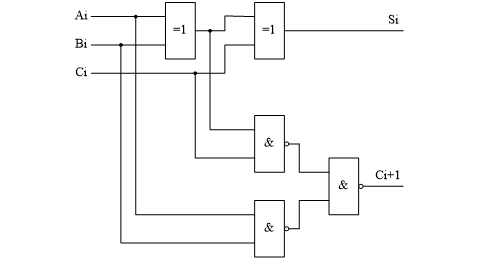
\includegraphics[width=3in]{H:/电子技术试验/4-19/4-19-7.png}
  \caption{全加器} \label{fig:aa}
\end{figure}
\begin{figure}[h]
  %\small
  \centering
  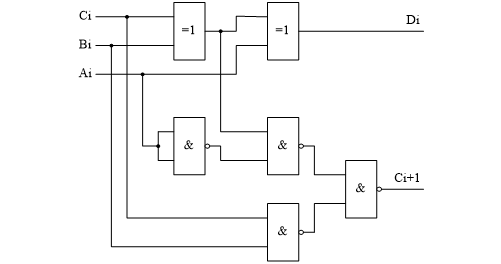
\includegraphics[width=3in]{H:/电子技术试验/4-19/4-19-8.png}
  \caption{全减器} \label{fig:aa}
  \end{figure}
\begin{figure}[h]
  %\small
  \centering
  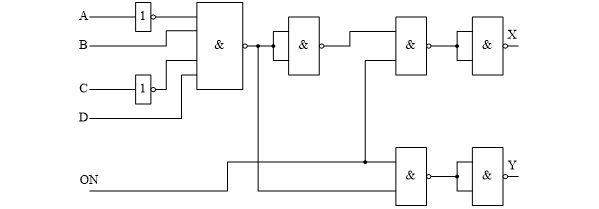
\includegraphics[width=3.5in]{H:/电子技术试验/4-19/4-19-9.png}
  \caption{保险箱四位密码锁} \label{fig:aa}
  \end{figure}
  
\newpage
\section{\zihao{4} 实验内容及步骤}
(1)分别按图1、2接线\par
(2)按照1验证全加器和全减器的逻辑功能\par
(2)设计保险箱四位密码锁电路,接线,并验证是否能够实现目标功能      \par




\section{\zihao{4} 数据及误差处理}
\subsection{全加器的逻辑功能}
\begin{table}[h]
  \centering  
  \begin{tabular}{c|c|c|c|c}
      \hline
      \multicolumn{3}{c}{输入} \vline  &  \multicolumn{2}{c}{输出} \vline     \\ \hline
            A             & B    &$C_i $   &  Si               & $ C_{i+1} $  \\ \hline
            0             & 0    &0        &   0               & 0            \\ \hline
            0             & 0    &1        &   1               & 0            \\ \hline
            0             & 1    &0        &   1               & 0            \\ \hline
            0             & 1    &1        &   0               & 1            \\ \hline
            1             & 0    &0        &   1               & 0            \\ \hline
            1             & 0    &1        &   0               & 1            \\ \hline
            1             & 1    &0        &   0               & 1            \\ \hline
            1             & 1    &1        &   1               & 1            \\ \hline
          \end{tabular}
\end{table}
\subsection{全减器的逻辑功能}
\begin{table}[h]
  \centering  
  \begin{tabular}{c|c|c|c|c}
      \hline
      \multicolumn{3}{c}{输入} \vline  &  \multicolumn{2}{c}{输出} \vline     \\ \hline
            A             & B    &$C_i $   &  Di               & $ C_{i+1} $  \\ \hline
            0             & 0    &0        &   0               & 0            \\ \hline
            0             & 0    &1        &   1               & 1            \\ \hline
            0             & 1    &0        &   1               & 1            \\ \hline
            0             & 1    &1        &   0               & 1            \\ \hline
            1             & 0    &0        &   1               & 0            \\ \hline
            1             & 0    &1        &   0               & 0            \\ \hline
            1             & 1    &0        &   0               & 0            \\ \hline
            1             & 1    &1        &   1               & 1            \\ \hline
          \end{tabular}
 \end{table}
 \subsection{四位密码锁设计}
 经实验验证,设计的密码锁能够实现目标功能




	\section{\zihao{4} 实验设备和器材}
	(1)直流稳压电源             \qquad \quad \qquad \qquad \qquad \qquad           1台\par
	(2)数字逻辑实验箱            \qquad  \qquad \qquad \qquad\qquad                1台\par
	(3)集成四-2输入与非门(74LS00) \qquad    \quad                                    2片\par
  (4)集成二-4输入与非门(74LS20) \qquad    \quad                                    2片\par
  (5)集成四-2输入异或门(74LS86) \qquad    \quad                                    2片\par
 	(6)导线                 \quad    \qquad  \qquad \qquad \qquad \qquad \qquad \qquad  1只\par
  
\section{结论}
(1)全加器满足逻辑关系
\begin{align*}
  \ Si&=A'B'Ci+A'BCi'+AB'Ci'+ABCi=(A\bigoplus B)\bigoplus Ci\\
  \ C_{i+1}&=ACi+AB+BCi
\end{align*}
\par 

(1)全减器满足逻辑关系
\begin{align*}
  \ Si&=A'B'Ci+A'BCi'+AB'Ci'+ABCi=(A\bigoplus B)\bigoplus Ci\\
  \  C_{i+1}&=A'B+A'C+BC
\end{align*}
\par 
(3)设计的四位密码器密码为0101,其功能符合预期。
\section{思考}
(1)通过实验,你认为 SSI组合逻辑电路设计的关键步骤是什么?\par 
逻辑抽象;列些真值表;写出逻辑函数表达式并化简与变换;画出逻辑图\par  
(2)对于同一个命题,是否有不同的设计方案?试比较各自的优缺点。\par 
有不同的方案,优缺点主要表现在竞争冒险和器件成本上\par 
(3)如何设计保护电路,防止集成器件损坏?\par 
接入直流电源时注意方向和控制电压大小\par 
\newpage
\section{自主设计半加器和半减器}
\subsection{半加器}
半加器的真值表如下
\begin{table}[h]
 \centering  
 \begin{tabular}{c|c|c|c|c}
     \hline
     \multicolumn{3}{c}{输入} \vline  &  \multicolumn{2}{c}{输出} \vline     \\ \hline
           A             & B     &  Si               & $ C_{i+1} $  \\ \hline
           0             & 0     &   0               & 0            \\ \hline
           0             & 1     &   1               & 0            \\ \hline
           1             & 0     &   1               & 0            \\ \hline
           1             & 1     &   0               & 1            \\ \hline
          \end{tabular}
\end{table}
\par
由此得到半加器的逻辑表达式如下
\begin{align*}
\ Di&=A'B+AB'=A\bigoplus B\\
\ C_{i+1}&=AB
\end{align*}
\par
由此得到半加器的逻辑电路图如下
\begin{figure}[h]
%\small
\centering
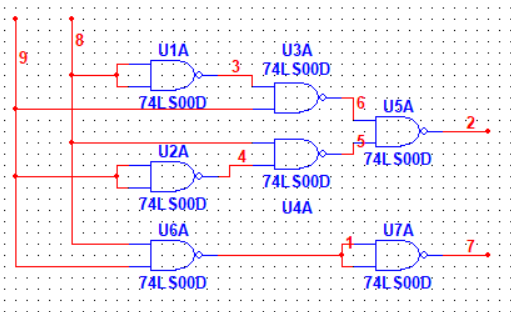
\includegraphics[width=4in]{H:/电子技术试验/4-19/4-19-1.png}
\caption{半加器} \label{fig:aa}
\end{figure}

\newpage
进行仿真,结果如下

\begin{figure}[h]
  %\small
  \centering
  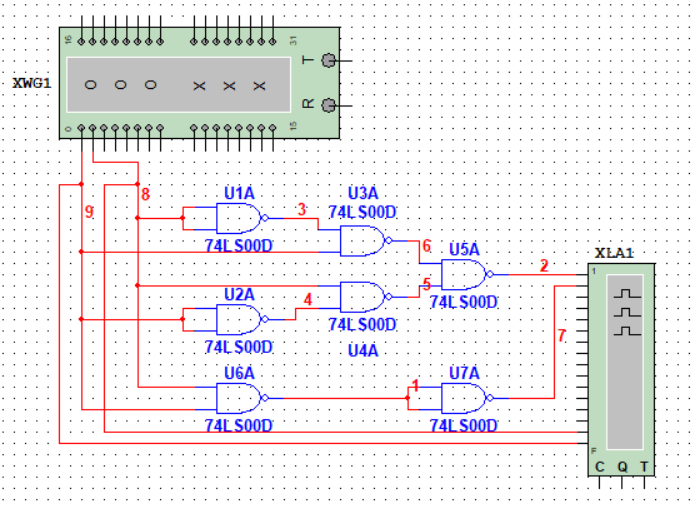
\includegraphics[width=4in]{H:/电子技术试验/4-19/4-19-2.png}
  \caption{半加器仿真电路} \label{fig:aa}
  \end{figure}
  \begin{figure}[h]
    %\small
    \centering
    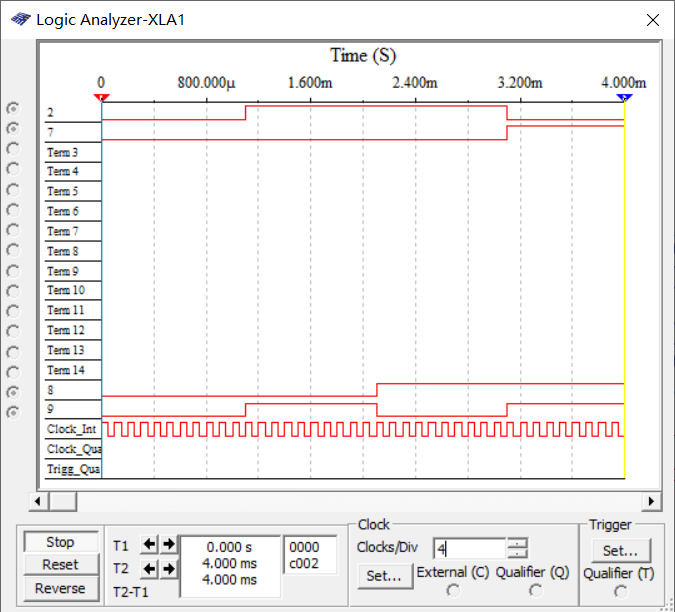
\includegraphics[width=3in]{H:/电子技术试验/4-19/4-19-3.png}
    \caption{仿真时序图} \label{fig:aa}
    \end{figure}

    \newpage
\subsection{半减器}
半减器的真值表如下
\begin{table}[h]
 \centering  
 \begin{tabular}{c|c|c|c|c}
     \hline
     \multicolumn{3}{c}{输入} \vline  &  \multicolumn{2}{c}{输出} \vline     \\ \hline
           A             & B     &  Di               & $ C_{i+1} $  \\ \hline
           0             & 0     &   0               & 0            \\ \hline
           0             & 1     &   1               & 1            \\ \hline
           1             & 0     &   1               & 0            \\ \hline
           1             & 1     &   0               & 0            \\ \hline
          \end{tabular}
\end{table}
\par
由此得到半减器的逻辑表达式如下
\begin{align*}
\ Di&=A'B+AB'=A\bigoplus B\\
\ C_{i+1}&=A'B
\end{align*}
\par
由此得到半减器的逻辑电路图如下
\begin{figure}[h]
%\small
\centering
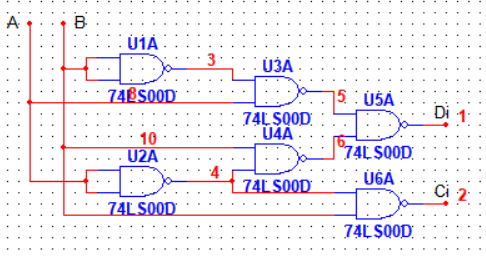
\includegraphics[width=4in]{H:/电子技术试验/4-19/4-19-5.png}
\caption{半减器} \label{fig:aa}
\end{figure}
\par 
\newpage
进行仿真,结果如下
\begin{figure}[h]
  %\small
  \centering
  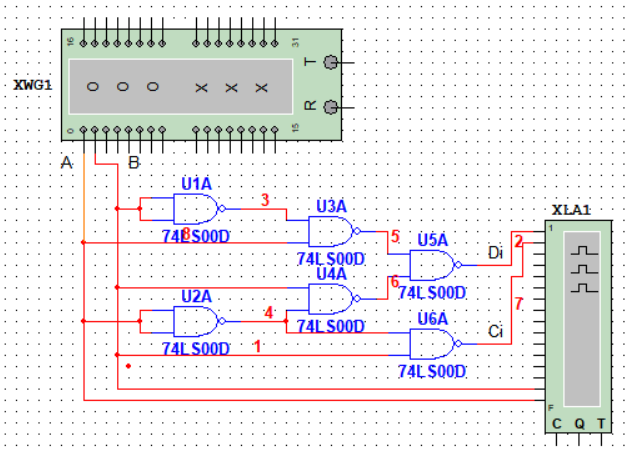
\includegraphics[width=4in]{H:/电子技术试验/4-19/4-19-4.png}
  \caption{半减器仿真电路} \label{fig:aa}
  \end{figure}
  \begin{figure}[h]
    %\small
    \centering
    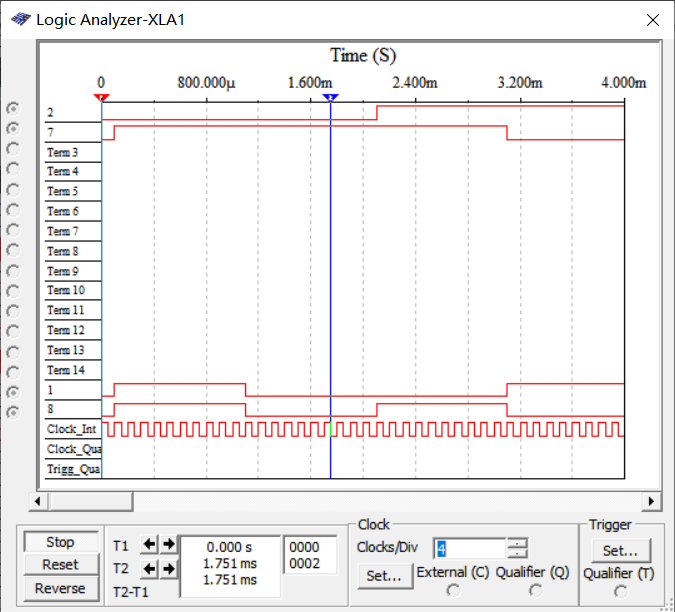
\includegraphics[width=3in]{H:/电子技术试验/4-19/4-19-6.png}
    \caption{仿真时序图} \label{fig:aa}
    \end{figure}
\end{document}